\chapter{Measured improvements}
\label{sec:improvements}

After implementing the transformations, we measure the effectiveness of the new normalization strategy. We look at the results from the perspective of submission coverage and normalization effectiveness.

\section{Submission coverage}

FIXME: explain what this is

% THEN: add charts

\begin{figure}
\centering
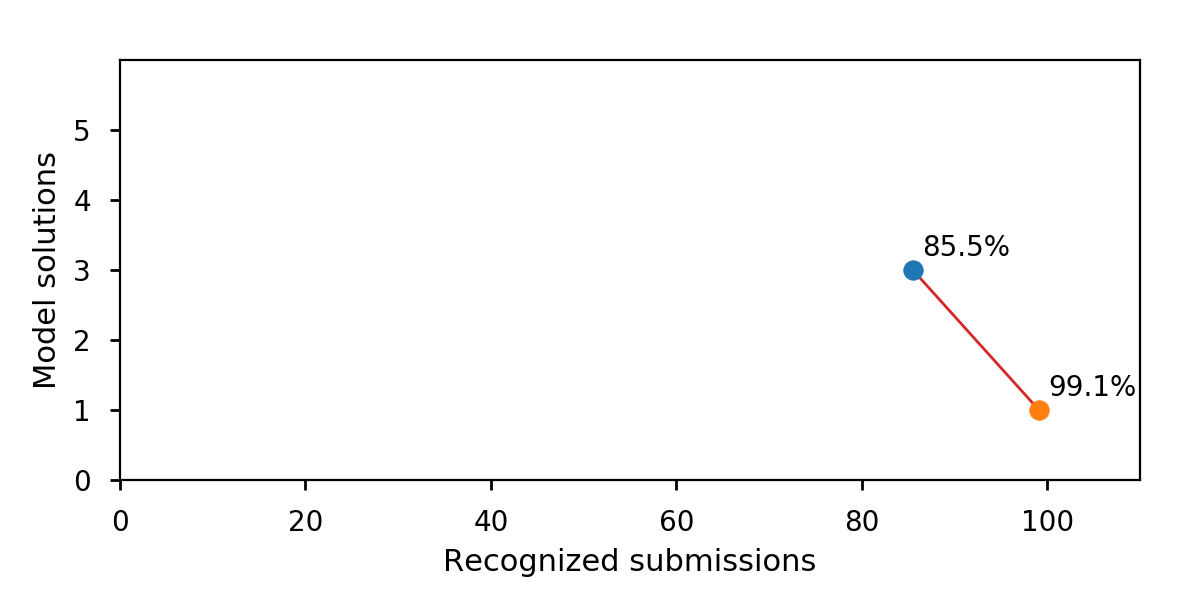
\includegraphics[height=5cm]{graphs/coverage-1.png}
\caption{Exercise 1 - Improvement in submission coverage}
\label{fig:improvements-coverage-1}
\end{figure}

\begin{figure}
\centering
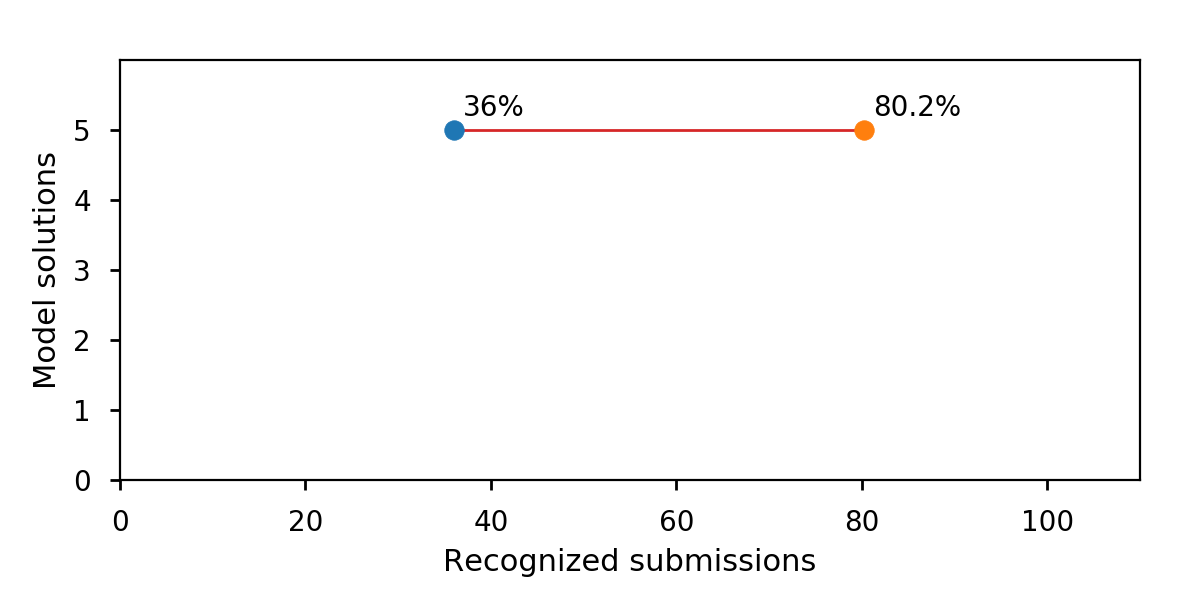
\includegraphics[height=5cm]{graphs/coverage-2.png}
\caption{Exercise 2 - Improvement in submission coverage}
\label{fig:improvements-coverage-2}
\end{figure}

\begin{figure}
\centering
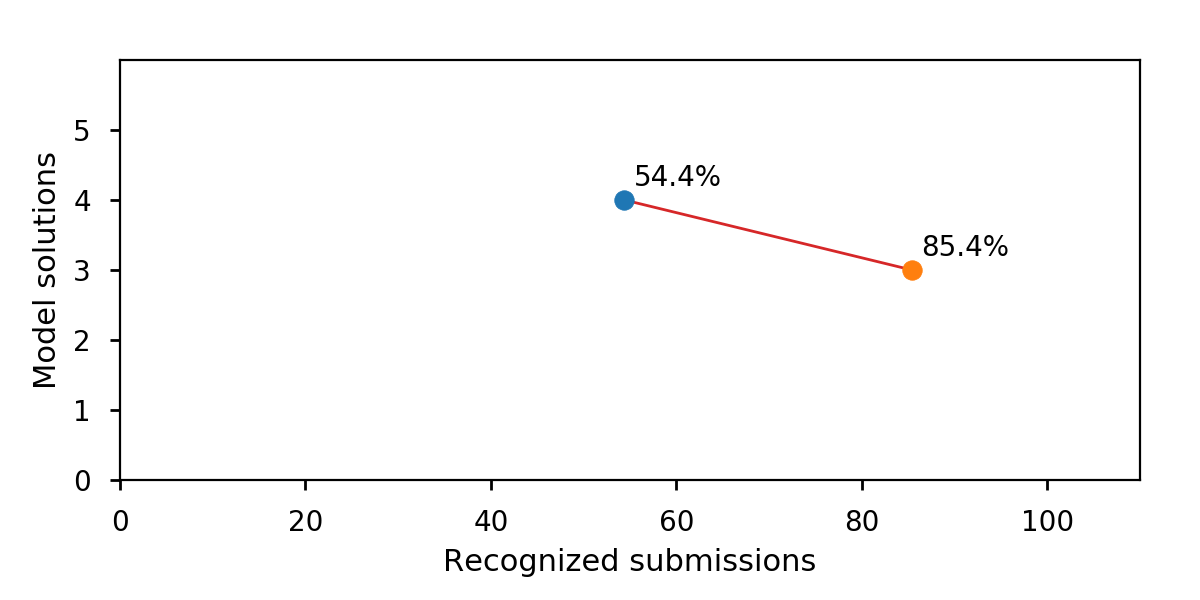
\includegraphics[height=5cm]{graphs/coverage-3.png}
\caption{Exercise 3 - Improvement in submission coverage}
\label{fig:improvements-coverage-3}
\end{figure}

\begin{figure}
\centering
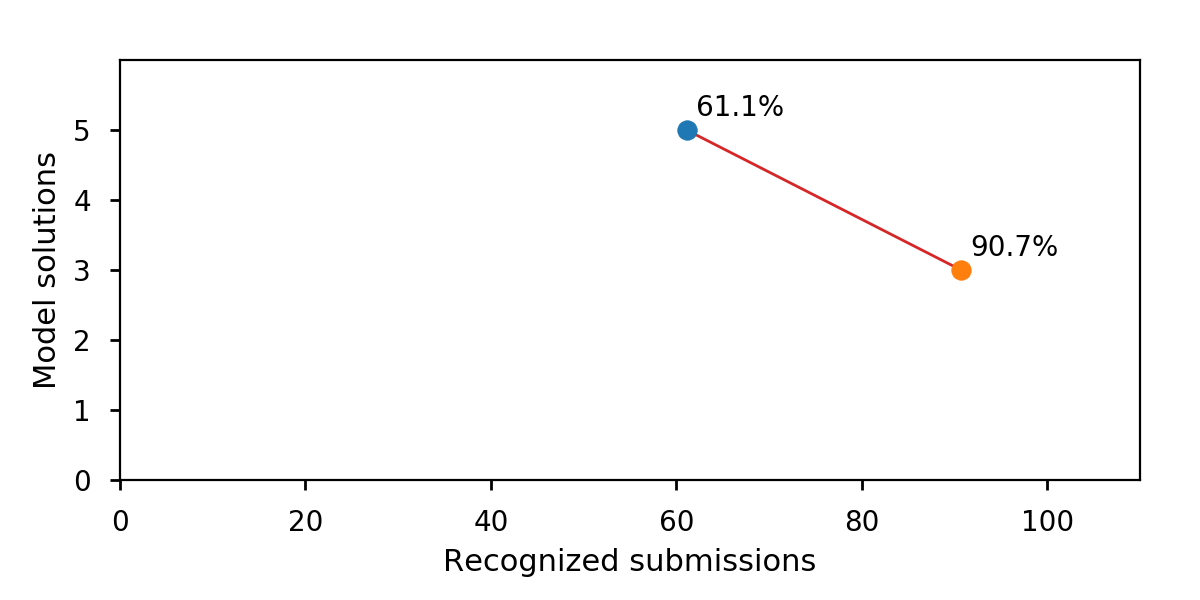
\includegraphics[height=5cm]{graphs/coverage-4.png}
\caption{Exercise 4 - Improvement in submission coverage}
\label{fig:improvements-coverage-4}
\end{figure}

\begin{figure}
\centering
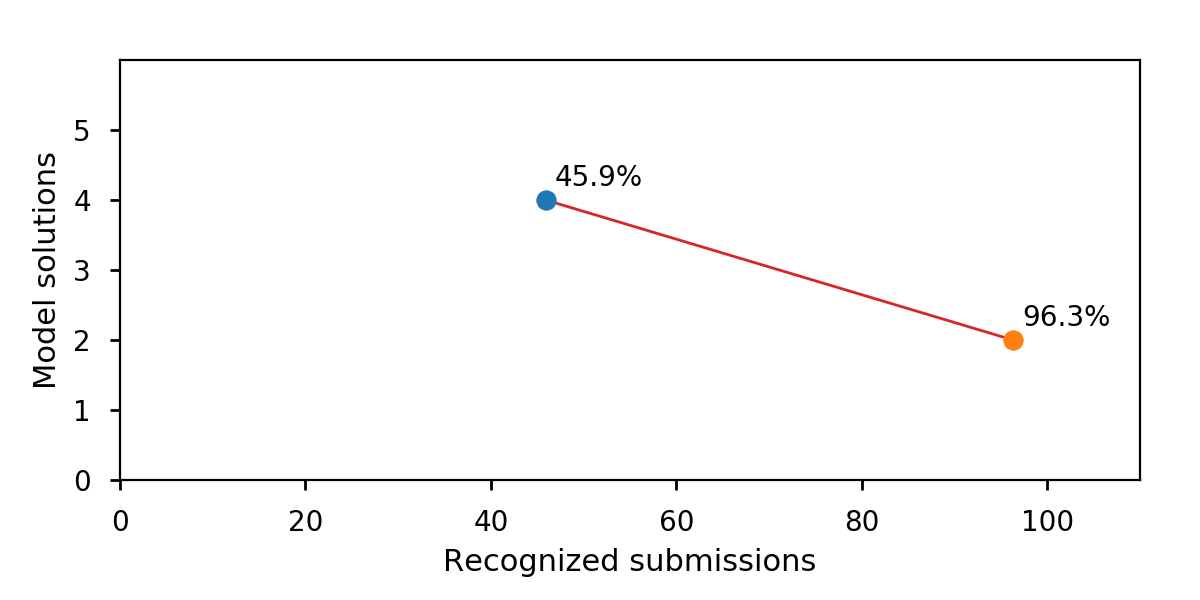
\includegraphics[height=5cm]{graphs/coverage-5.png}
\caption{Exercise 5 - Improvement in submission coverage}
\label{fig:improvements-coverage-5}
\end{figure}

\begin{figure}
\centering
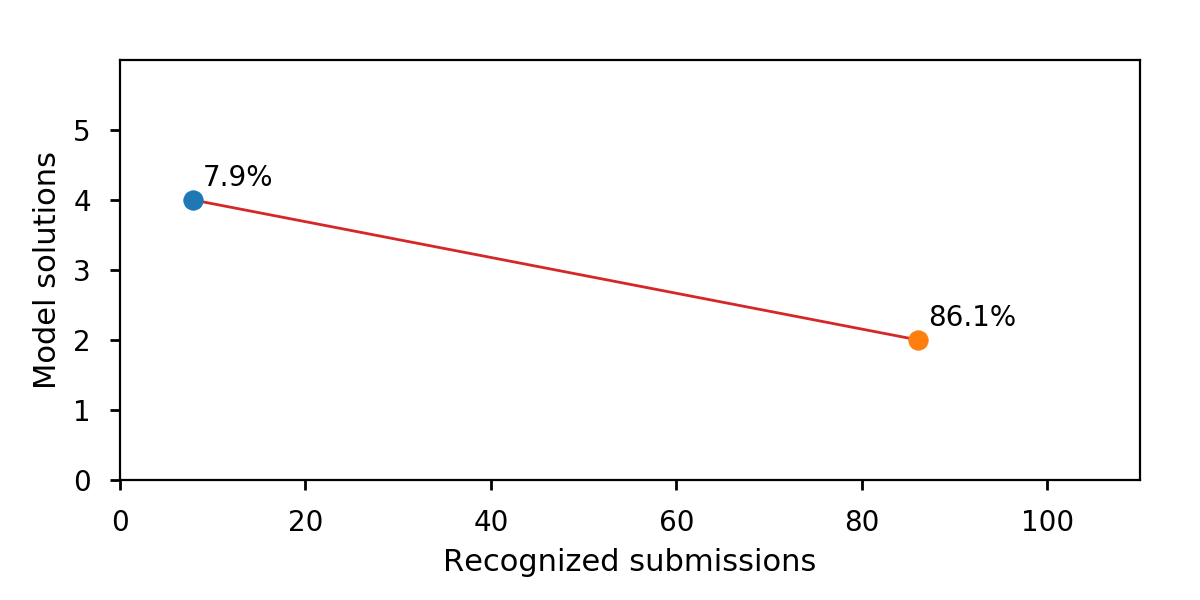
\includegraphics[height=5cm]{graphs/coverage-6.png}
\caption{Exercise 6 - Improvement in submission coverage}
\label{fig:improvements-coverage-6}
\end{figure}

\begin{figure}
\centering
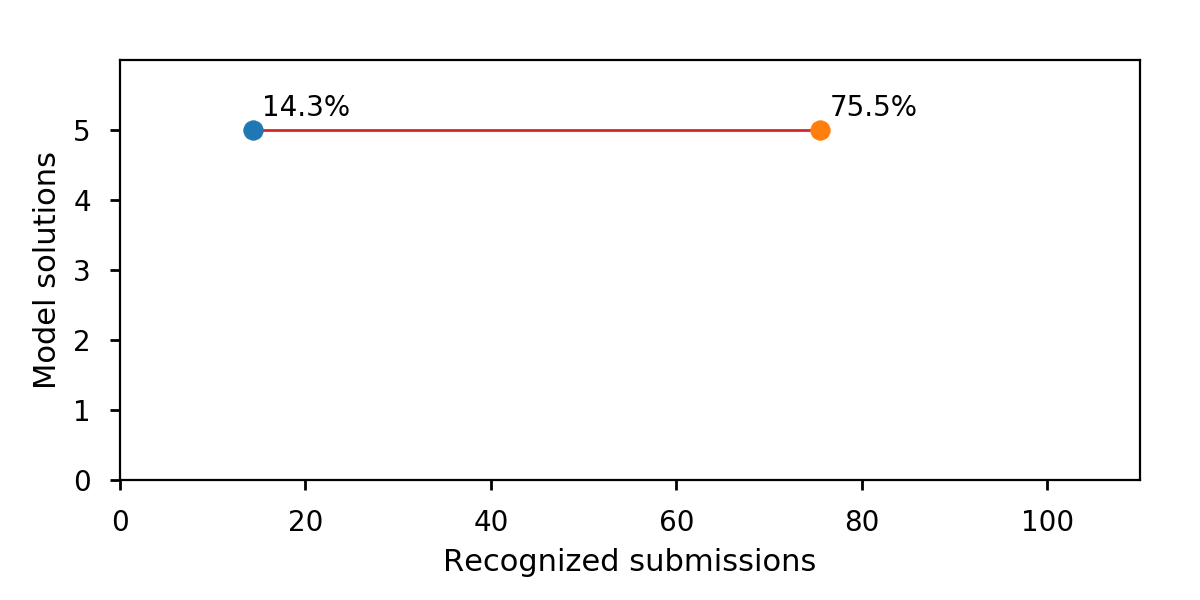
\includegraphics[height=5cm]{graphs/coverage-7.png}
\caption{Exercise 7 - Improvement in submission coverage}
\label{fig:improvements-coverage-7}
\end{figure}

\begin{figure}
\centering
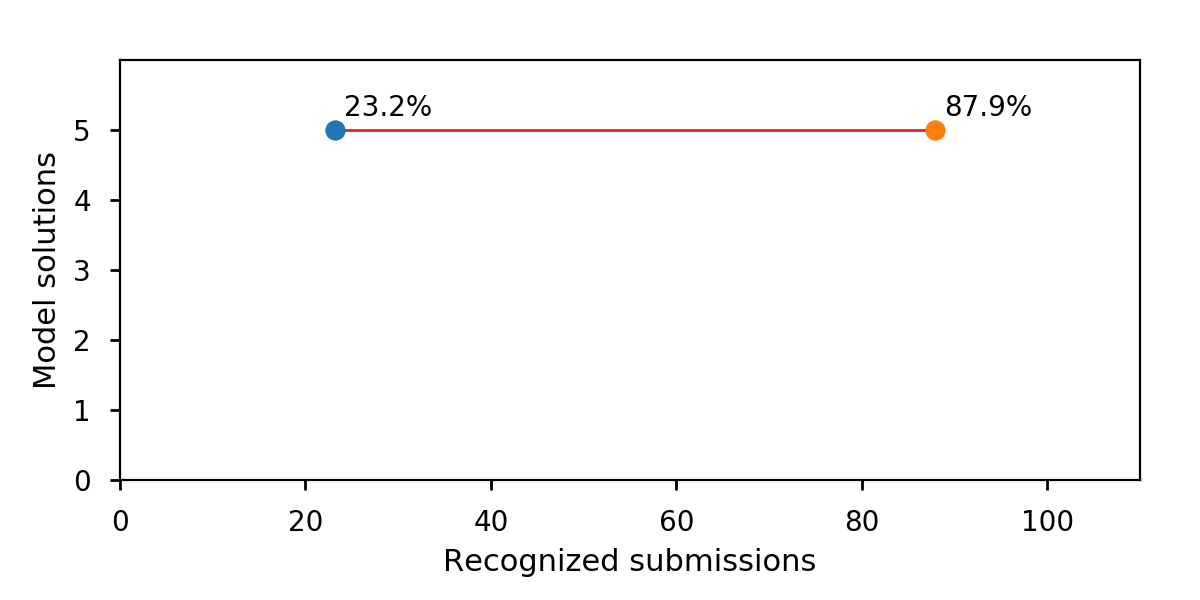
\includegraphics[height=5cm]{graphs/coverage-8.png}
\caption{Exercise 8 - Improvement in submission coverage}
\label{fig:improvements-coverage-8}
\end{figure}

% \begin{itemize}
%     \item Exercise 1: from 85.5\% with 3 model solutions to 99.1\% with 1 model solution.
%     \item Exercise 2: from 36\% with 5 model solutions to 80.2\% with 5 model solutions.
%     \item Exercise 3: from 54.4\% with 4 model solutions to 85.4\% with 3 model solutions.
%     \item Exercise 4: from 61.1\% with 5 model solutions to 90.7\% with 3 model solutions.
%     \item Exercise 5: from 45\% with 4 model solutions to 96.4\% with 2 model solutions.
%     \item Exercise 6: from 7.9\% with 4 model solutions to 86.1\% with 2 model solutions.
%     \item Exercise 7: from 14.1\% with 5 model solutions to 74.7\% with 5 model solutions.
%     \item Exercise 8: from 23.2\% with 5 model solutions to 87.9\% with 5 model solutions.
% \end{itemize}

\section{Normalization effectiveness}

FIXME: explain what this is

% THEN: add charts

\begin{figure}
\centering
\begin{tabular}{ >{\centering\arraybackslash}m{14em} >{\centering\arraybackslash}m{14em} }
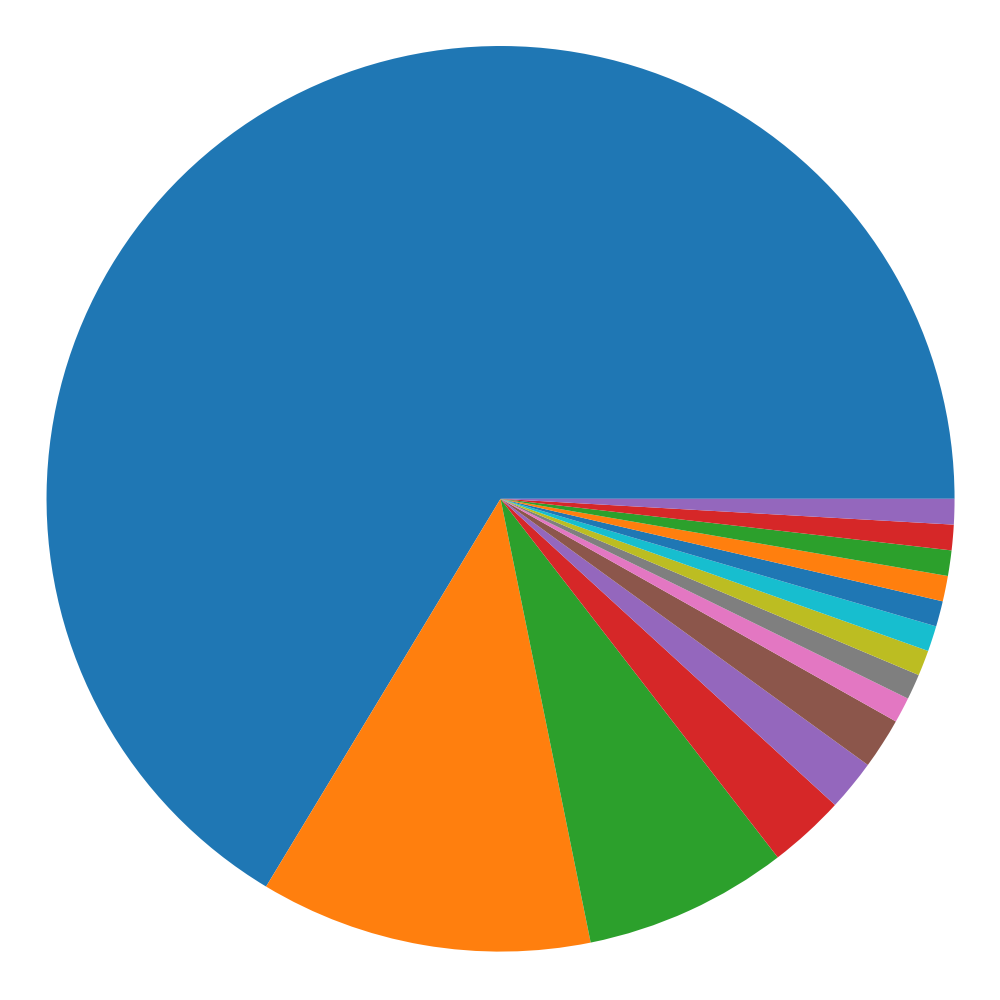
\includegraphics[height=5cm]{graphs/cluster-baseline-1.png}
&
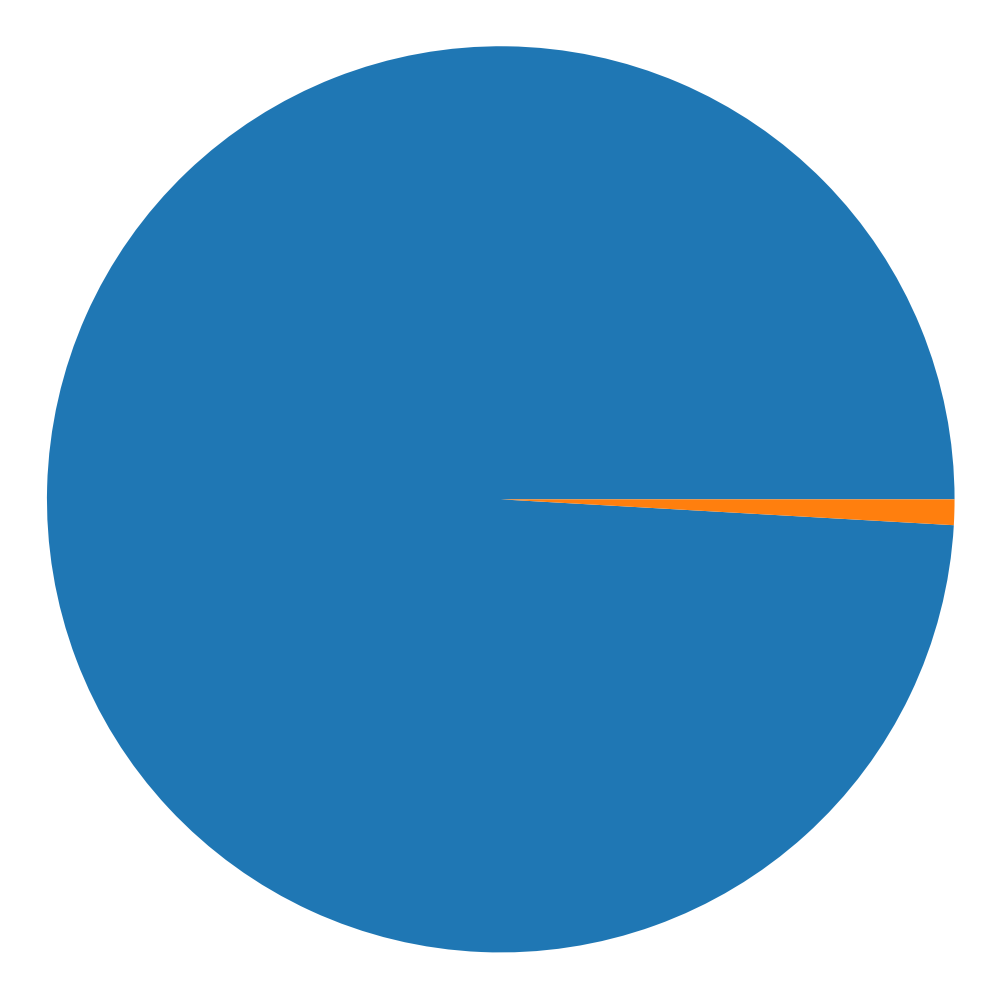
\includegraphics[height=5cm]{graphs/cluster-aggressive-1.png} \\
Before & After
\end{tabular}
\caption{Exercise 1 - Improvement in normalization effectiveness}
\label{fig:improvements-clusters-1}
\end{figure}

\begin{figure}
\centering
\begin{tabular}{ >{\centering\arraybackslash}m{14em} >{\centering\arraybackslash}m{14em} }
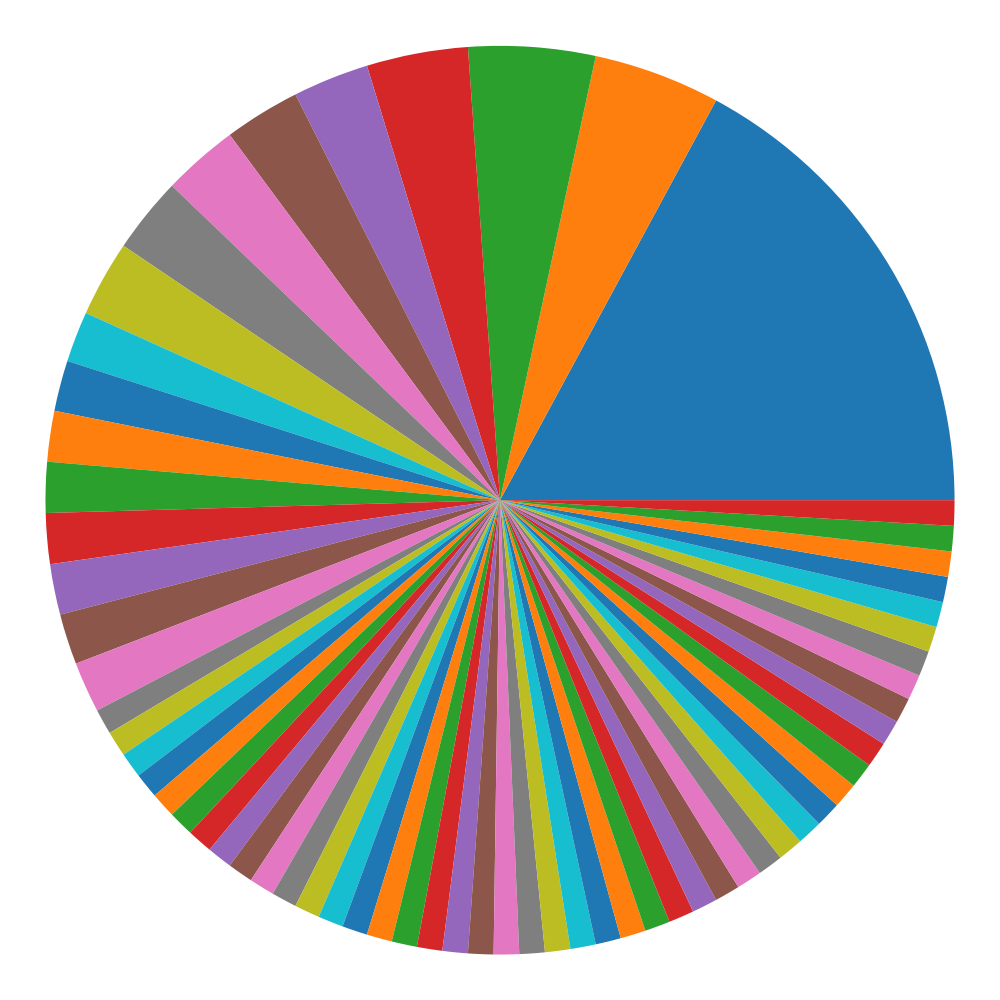
\includegraphics[height=5cm]{graphs/cluster-baseline-2.png}
&
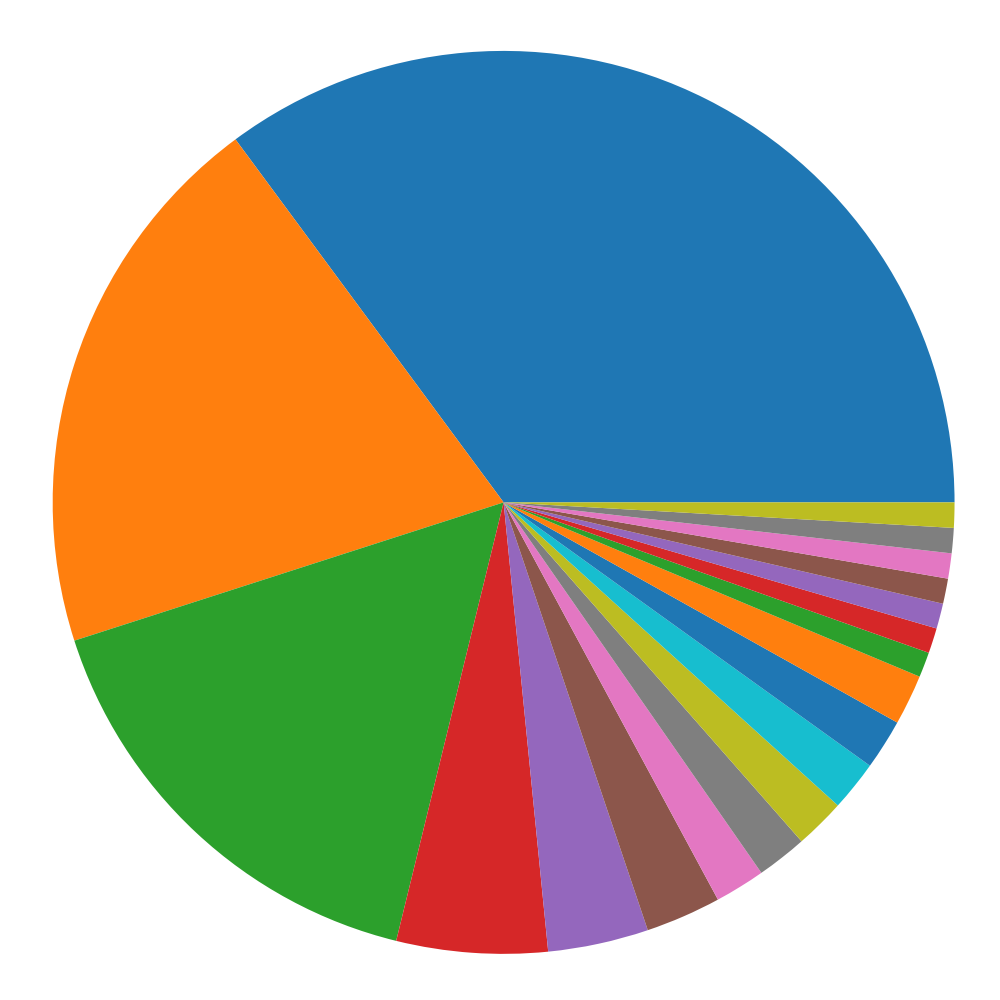
\includegraphics[height=5cm]{graphs/cluster-aggressive-2.png} \\
Before & After
\end{tabular}
\caption{Exercise 2 - Improvement in normalization effectiveness}
\label{fig:improvements-clusters-2}
\end{figure}

\begin{figure}
\centering
\begin{tabular}{ >{\centering\arraybackslash}m{14em} >{\centering\arraybackslash}m{14em} }
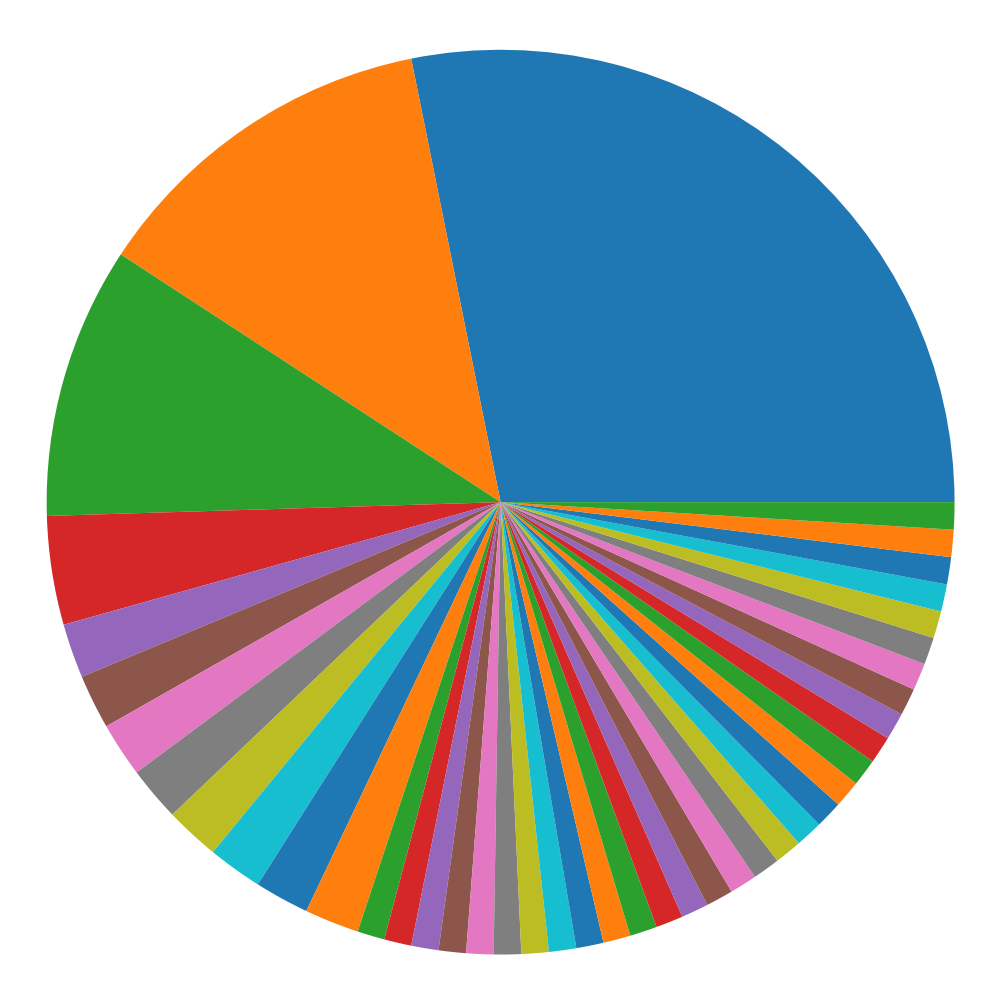
\includegraphics[height=5cm]{graphs/cluster-baseline-3.png}
&
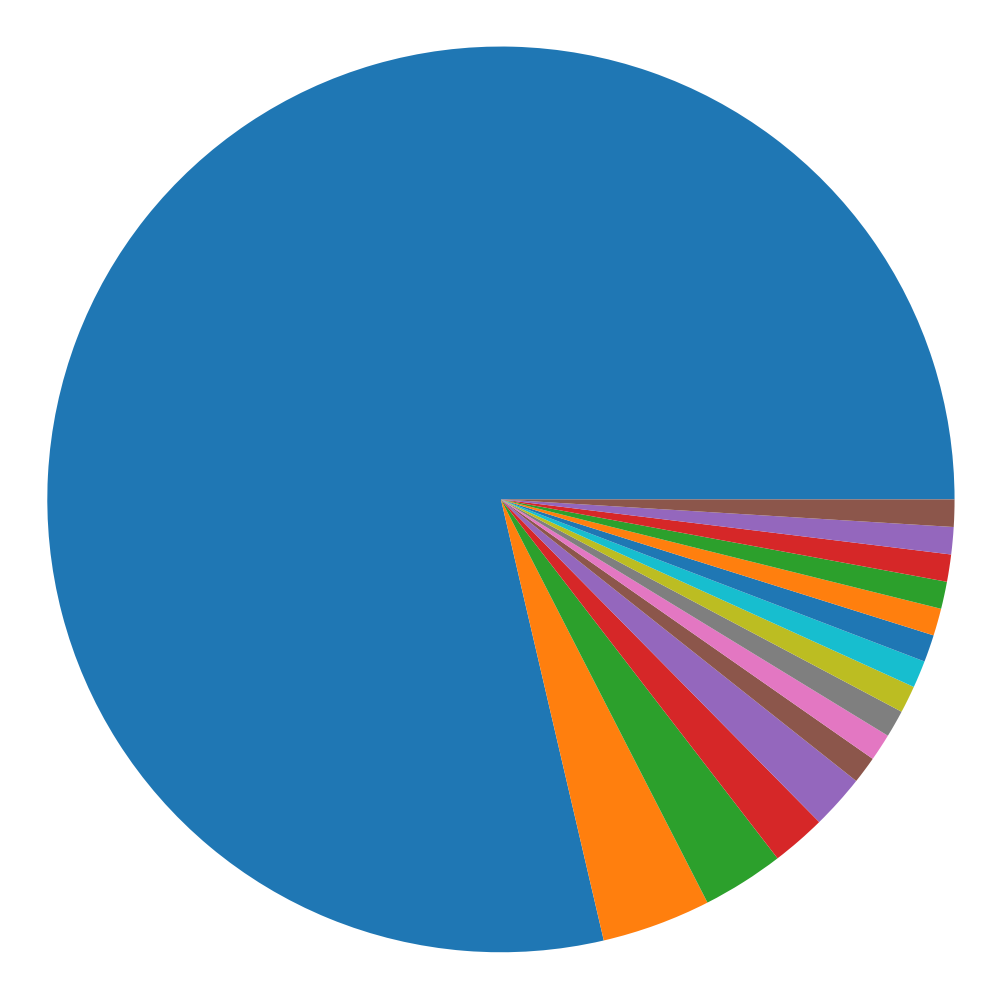
\includegraphics[height=5cm]{graphs/cluster-aggressive-3.png} \\
Before & After
\end{tabular}
\caption{Exercise 3 - Improvement in normalization effectiveness}
\label{fig:improvements-clusters-3}
\end{figure}

\begin{figure}
\centering
\begin{tabular}{ >{\centering\arraybackslash}m{14em} >{\centering\arraybackslash}m{14em} }
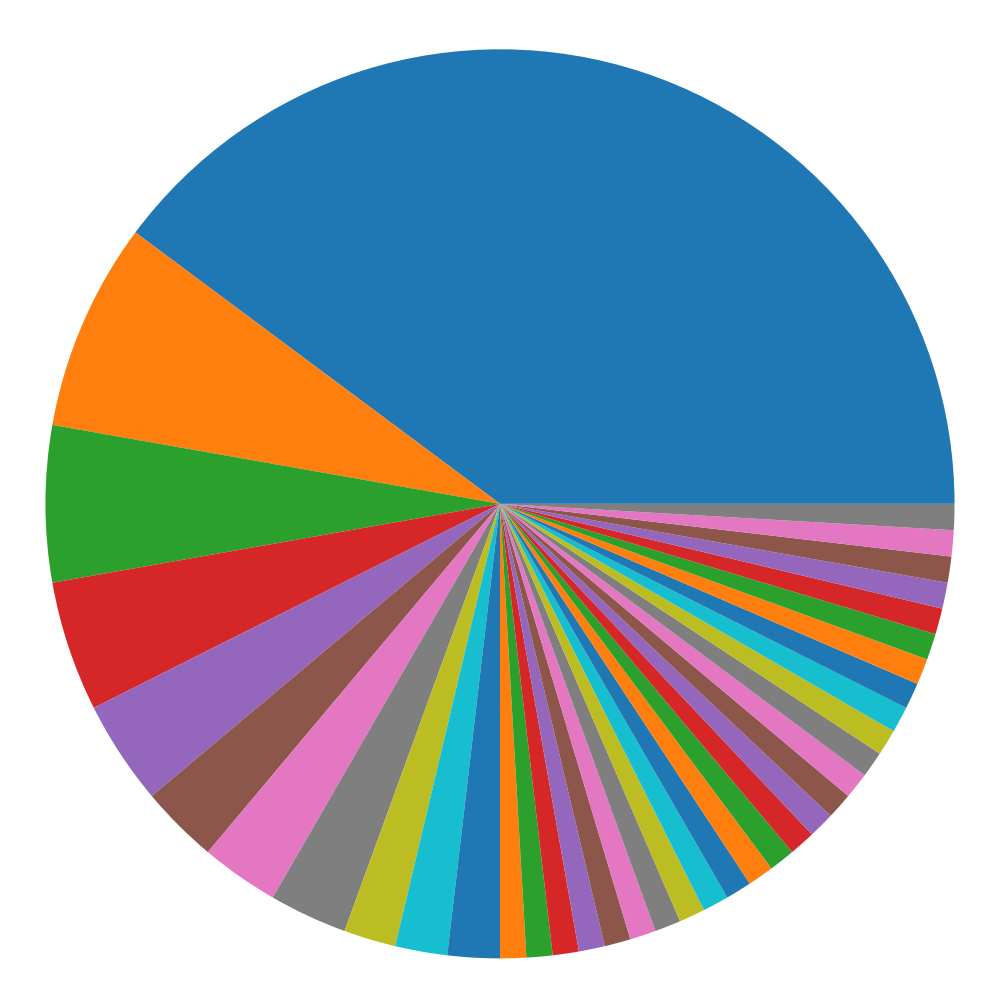
\includegraphics[height=5cm]{graphs/cluster-baseline-4.png}
&
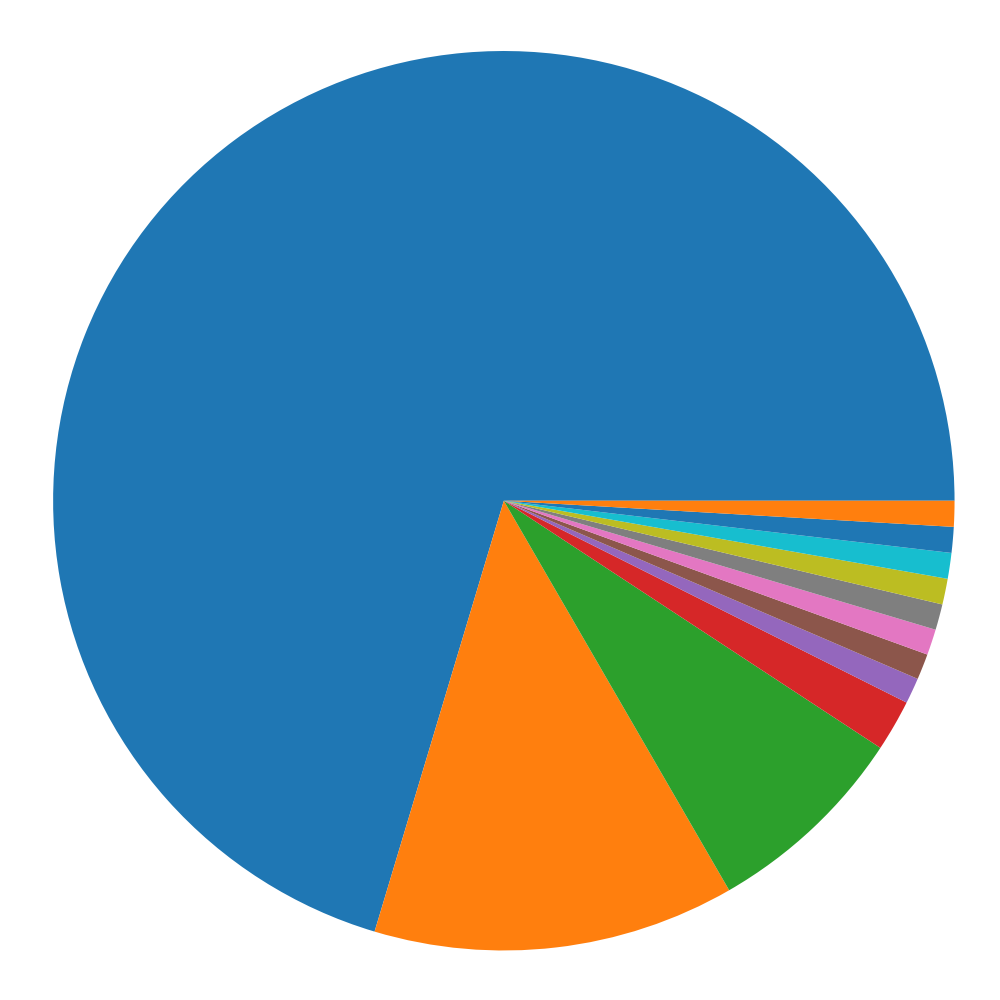
\includegraphics[height=5cm]{graphs/cluster-aggressive-4.png} \\
Before & After
\end{tabular}
\caption{Exercise 4 - Improvement in normalization effectiveness}
\label{fig:improvements-clusters-4}
\end{figure}

\begin{figure}
\centering
\begin{tabular}{ >{\centering\arraybackslash}m{14em} >{\centering\arraybackslash}m{14em} }
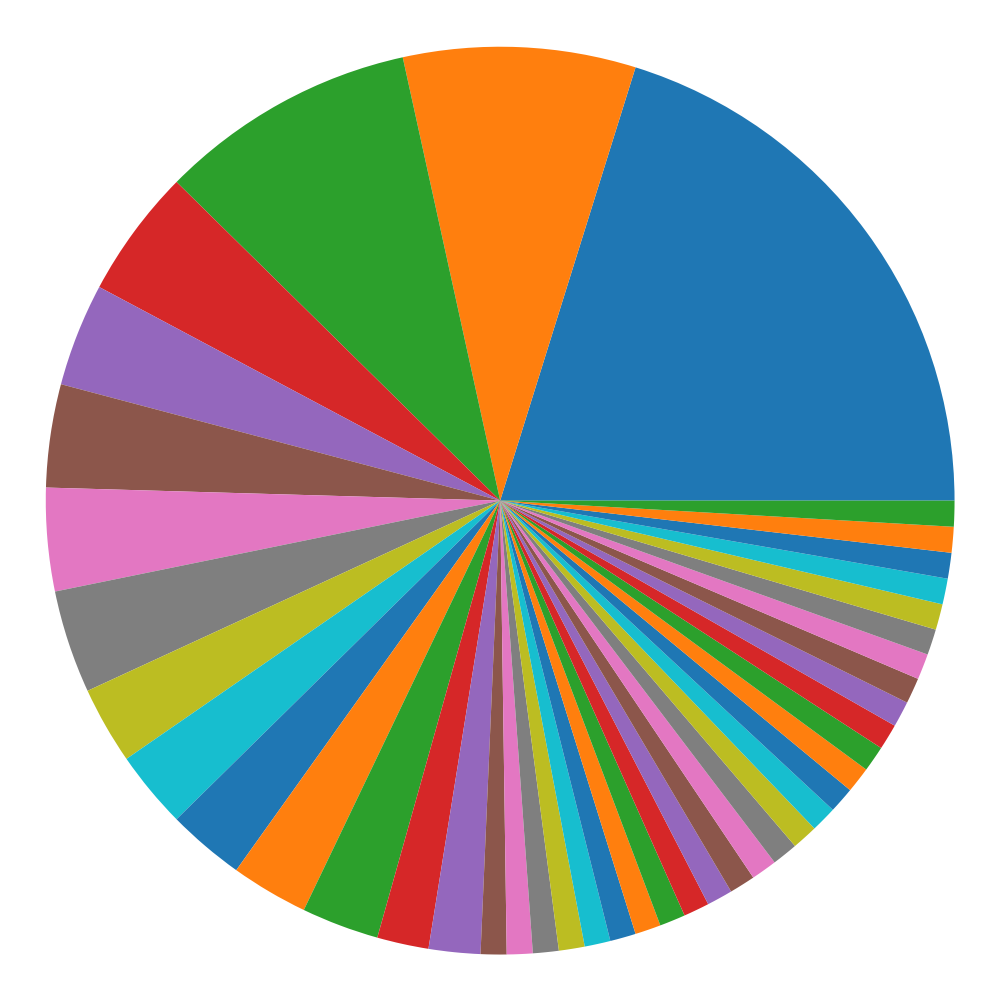
\includegraphics[height=5cm]{graphs/cluster-baseline-5.png}
&
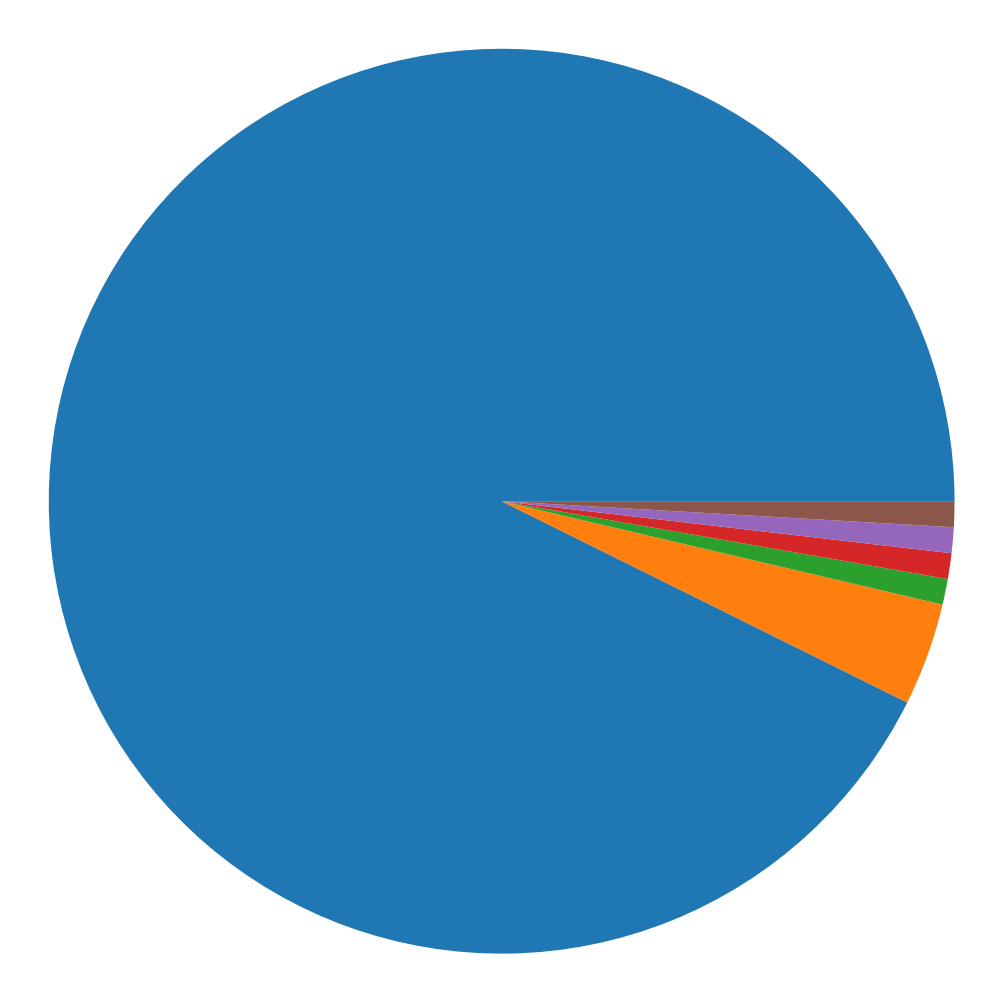
\includegraphics[height=5cm]{graphs/cluster-aggressive-5.png} \\
Before & After
\end{tabular}
\caption{Exercise 5 - Improvement in normalization effectiveness}
\label{fig:improvements-clusters-5}
\end{figure}

\begin{figure}
\centering
\begin{tabular}{ >{\centering\arraybackslash}m{14em} >{\centering\arraybackslash}m{14em} }
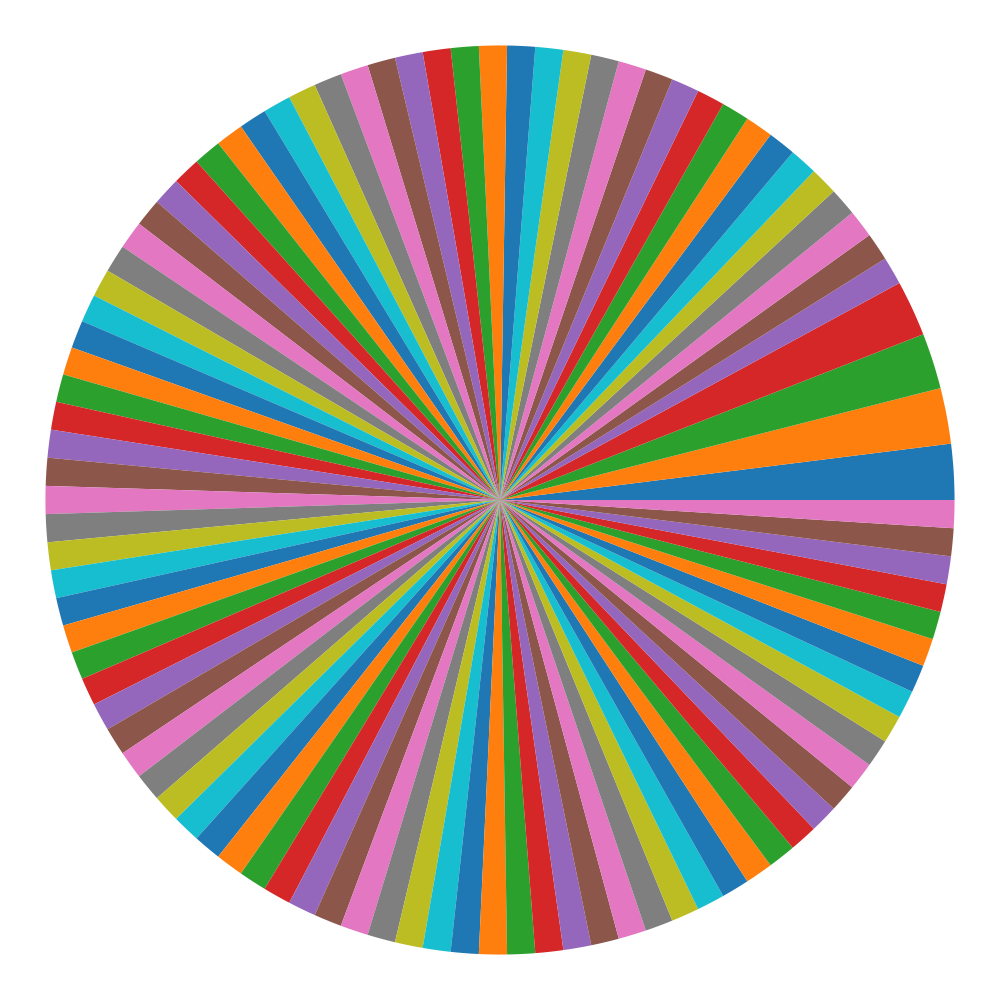
\includegraphics[height=5cm]{graphs/cluster-baseline-6.png}
&
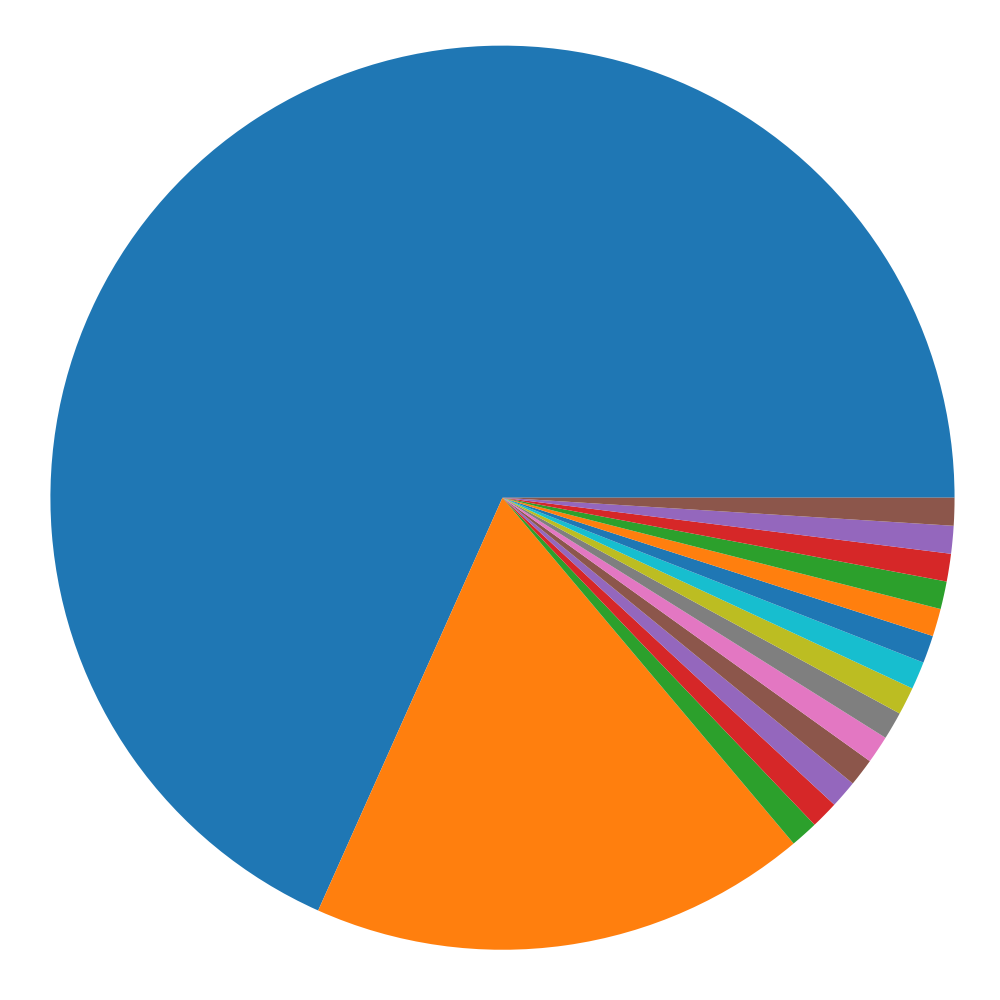
\includegraphics[height=5cm]{graphs/cluster-aggressive-6.png} \\
Before & After
\end{tabular}
\caption{Exercise 6 - Improvement in normalization effectiveness}
\label{fig:improvements-clusters-6}
\end{figure}

\begin{figure}
\centering
\begin{tabular}{ >{\centering\arraybackslash}m{14em} >{\centering\arraybackslash}m{14em} }
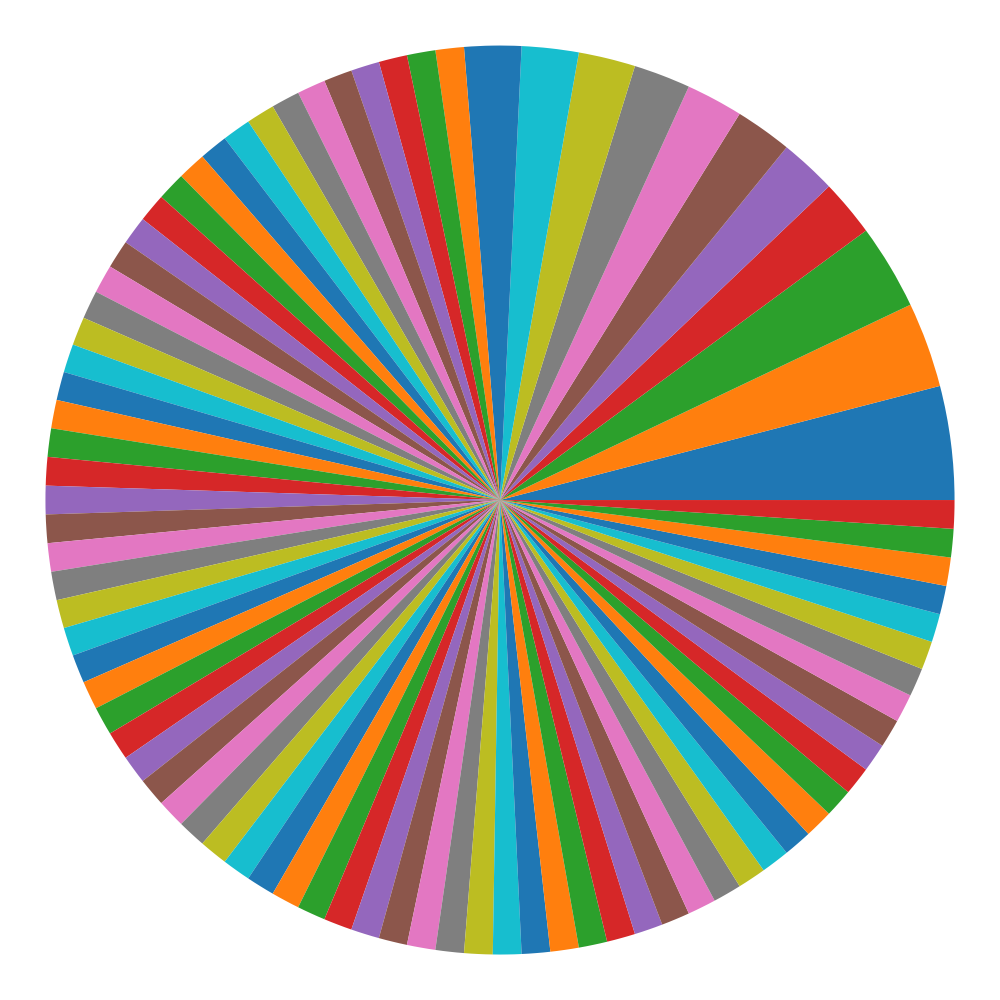
\includegraphics[height=5cm]{graphs/cluster-baseline-7.png}
&
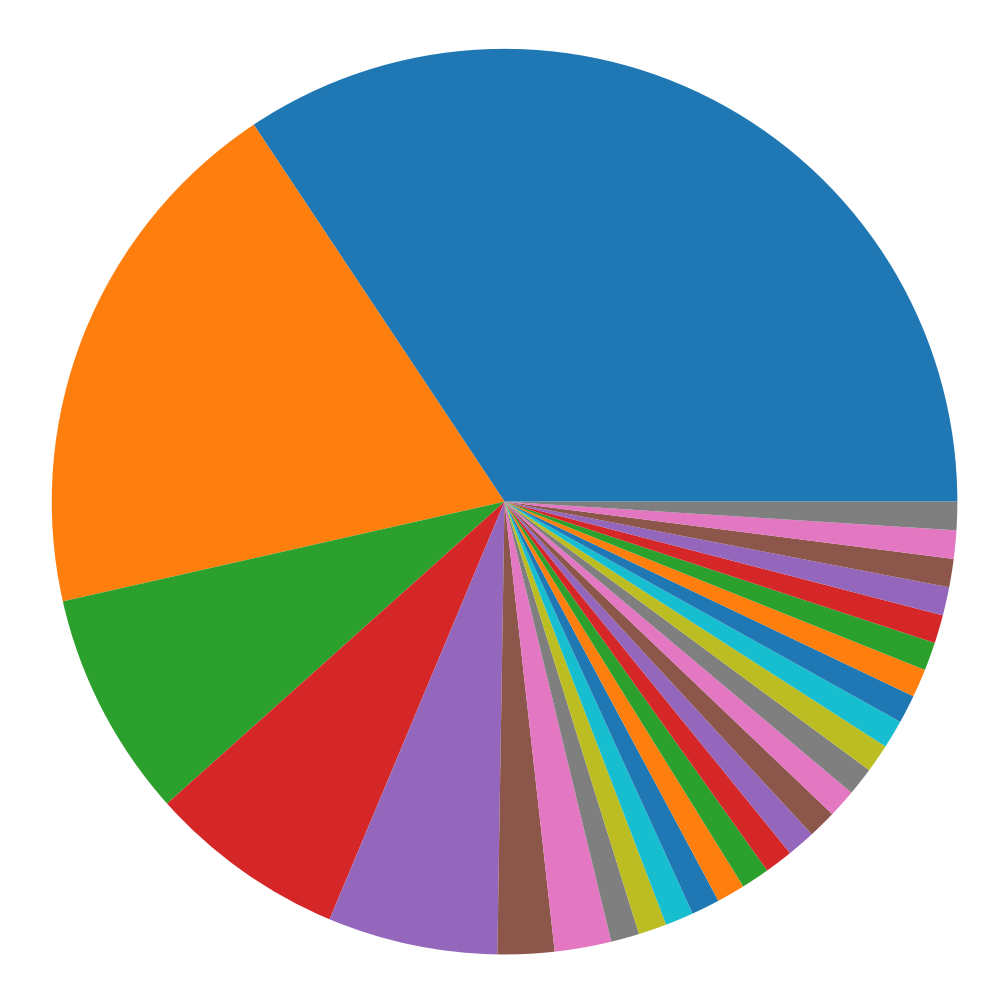
\includegraphics[height=5cm]{graphs/cluster-aggressive-7.png} \\
Before & After
\end{tabular}
\caption{Exercise 7 - Improvement in normalization effectiveness}
\label{fig:improvements-clusters-7}
\end{figure}

\begin{figure}
\centering
\begin{tabular}{ >{\centering\arraybackslash}m{14em} >{\centering\arraybackslash}m{14em} }
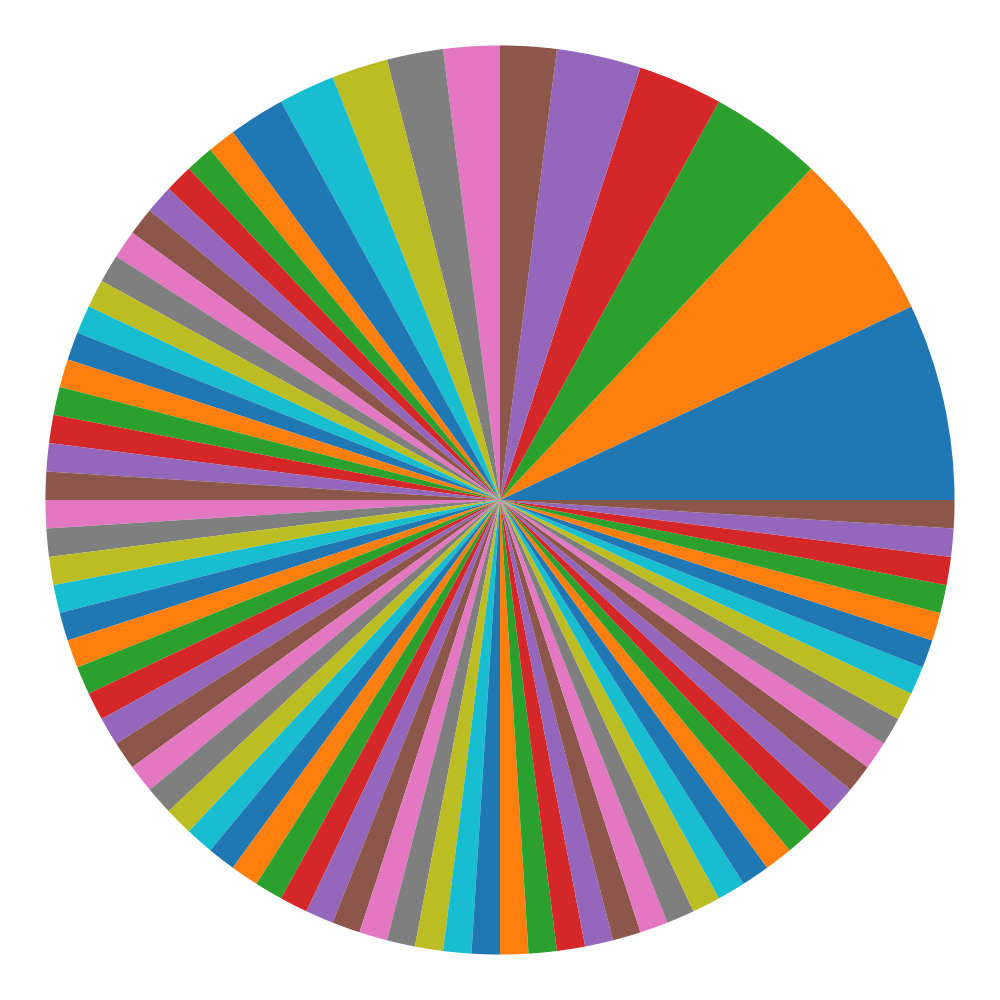
\includegraphics[height=5cm]{graphs/cluster-baseline-8.png}
&
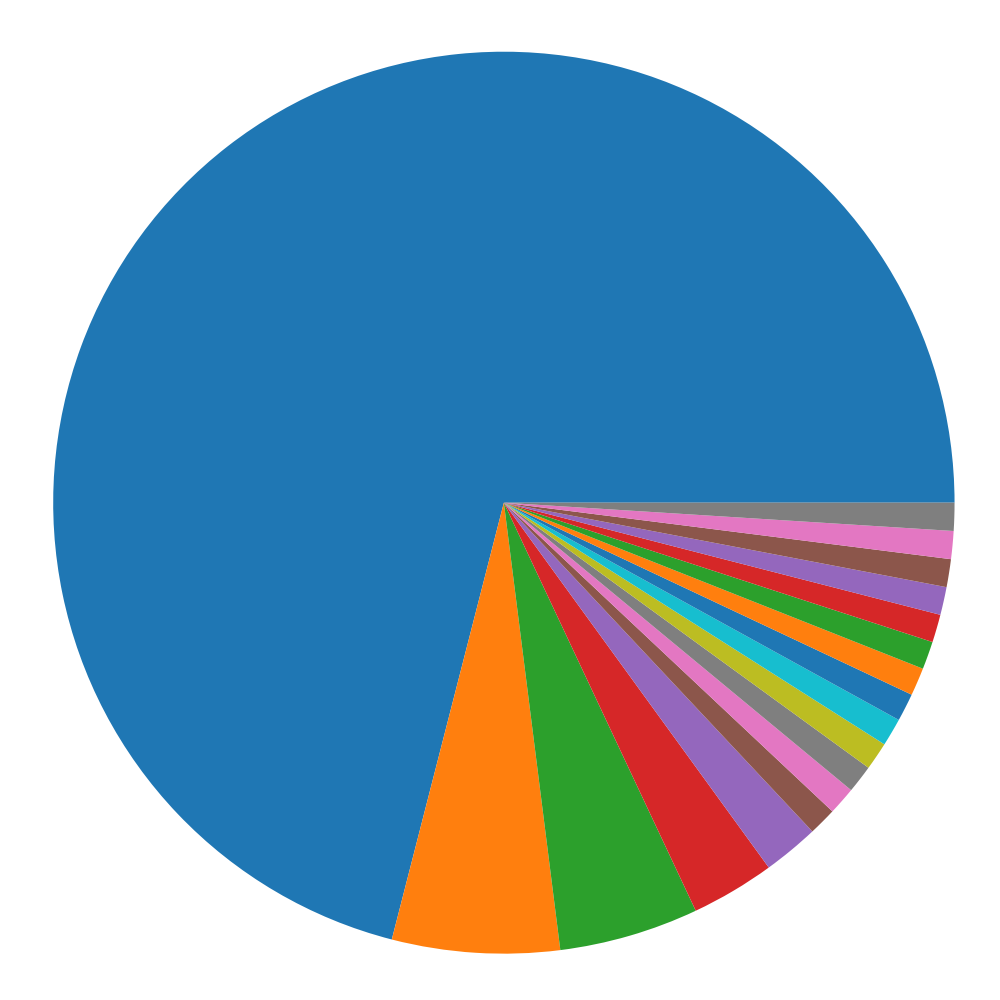
\includegraphics[height=5cm]{graphs/cluster-aggressive-8.png} \\
Before & After
\end{tabular}
\caption{Exercise 8 - Improvement in normalization effectiveness}
\label{fig:improvements-clusters-8}
\end{figure}
